\chapter{Sinusoidal Steady State and Impedance}\label{ch:b1:sinusoidal-impedance}

Turn the dial of an old radio and, out of the hundred stations that all
reach the antenna at once, one comes through: a coil and a variable
capacitor have been tuned so that exactly one frequency makes them
resonate. The mains that hums in every wall is a \qty{50}{Hz} sinusoid;
the factory that runs big motors on it pays a penalty if its current
lags its \omterm{def:b1:dc-circuits:voltage}{voltage} too much. Sinusoids are the natural language of
\omterm{def:b1:dc-circuits:linear}{linear circuits} --- they come out as they go in, only scaled and shifted
--- and this chapter gives them their algebra: \omterm{def:b1:sinusoidal-impedance:complex}{complex amplitudes},
\omterm{def:b1:sinusoidal-impedance:impedance}{impedances}, the resonance of the \omterm{prop:b1:transient-regimes:rlc}{RLC circuit}, and the power that
sinusoidal currents actually deliver.

\begin{omfigure}
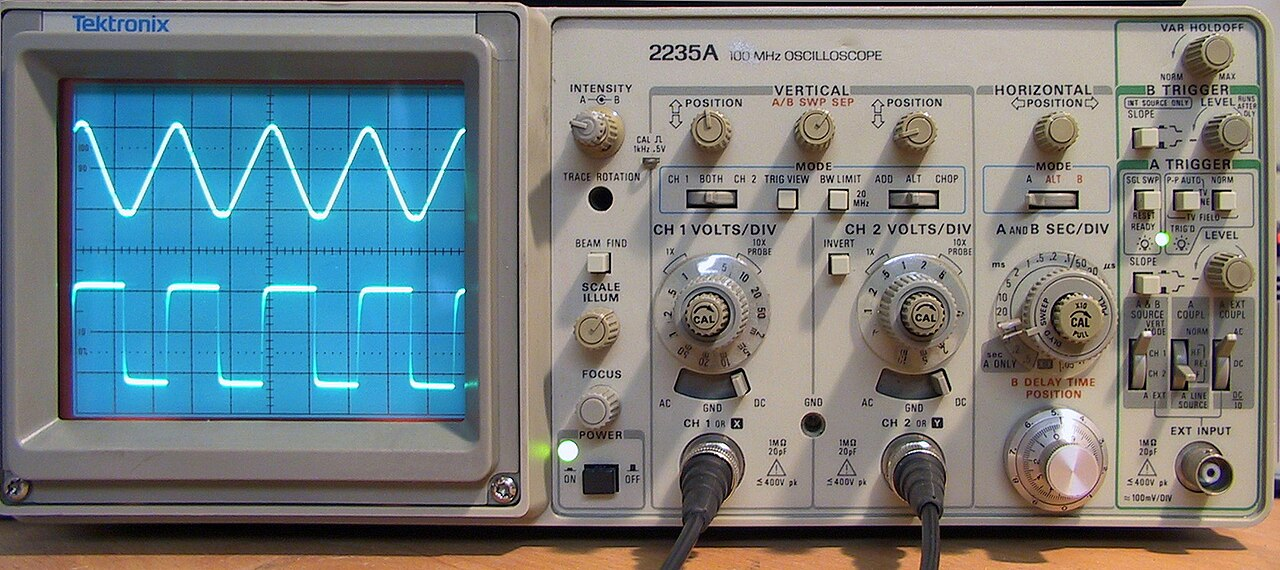
\includegraphics[width=0.60\linewidth]{images/book3/oscilloscope-sine-square.jpg}

{\small An oscilloscope showing a sinusoid and a square wave: the sinusoid is the \omterm{def:b1:wave-propagation:signal}{signal} this chapter lives on, the square wave the one the next chapter decomposes into sinusoids.}
\end{omfigure}

\section{The sinusoidal steady state}

\begin{proposition}[Forced sinusoidal regime]\label{prop:b1:sinusoidal-impedance:forced}
\index{sinusoidal steady state}\index{forced regime}
In a \omterm{def:b1:dc-circuits:linear}{linear circuit} driven by a sinusoidal source of \omterm{def:b1:wave-propagation:signal}{angular frequency}
$\omega$, every current and \omterm{def:b1:dc-circuits:voltage}{voltage} is, once the transients have died
out, a sinusoid of the same \omterm{def:b1:wave-propagation:signal}{angular frequency} $\omega$, each with its
own \omterm{def:b1:wave-propagation:signal}{amplitude} and phase: $x(t) = X\cos(\omega t + \varphi)$.
\end{proposition}

\begin{proof}
The circuit's equations are linear differential equations with constant
coefficients; their general solution is a particular solution plus the
solutions of the homogeneous equation, which are the transients of
\cref{ch:b1:transient-regimes} and decay (every real circuit has some
resistance). A sinusoidal particular solution exists because
differentiating a sinusoid of frequency $\omega$ gives a sinusoid of
the same frequency: the equations can be satisfied term by term --- the
complex method below constructs it explicitly.
\end{proof}

\begin{definition}[Complex amplitude]\label{def:b1:sinusoidal-impedance:complex}
\index{complex amplitude}\index{phasor}
To the sinusoid $x(t) = X\cos(\omega t + \varphi)$ one associates the
complex \omterm{def:b1:wave-propagation:signal}{signal} $\underline{x}(t) = X\eu^{j(\omega t + \varphi)}$, so that
$x = \Rea(\underline{x})$, and the \emph{complex \omterm{def:b1:wave-propagation:signal}{amplitude}}
\[
\underline{X} = X\eu^{j\varphi}, \qquad \underline{x}(t) = \underline{X}\,\eu^{j\omega t},
\]
which carries the \omterm{def:b1:wave-propagation:signal}{amplitude} $X = \abs{\underline{X}}$ and the phase
$\varphi = \arg\underline{X}$. Here $j$ denotes the imaginary unit,
$j^2 = -1$, the letter $i$ being reserved for currents. Drawn as a
vector of length $X$ at angle $\varphi$, $\underline{X}$ is a
\emph{phasor} (Fresnel vector).
\end{definition}

\begin{proposition}[Rules of the complex method]\label{prop:b1:sinusoidal-impedance:rules}
\begin{enumerate}
  \item Linear operations commute with taking the real part: the
        \omterm{def:b1:sinusoidal-impedance:complex}{complex amplitude} of a sum is the sum of the \omterm{def:b1:sinusoidal-impedance:complex}{complex amplitudes}.
  \item Differentiating with respect to time multiplies the \omterm{def:b1:sinusoidal-impedance:complex}{complex
        amplitude} by $j\omega$; integrating divides it by $j\omega$.
  \item \omterm{thm:b1:dc-circuits:kirchhoff}{Kirchhoff's laws}, being linear, hold for \omterm{def:b1:sinusoidal-impedance:complex}{complex amplitudes}.
\end{enumerate}
\end{proposition}

\begin{proof}
$\Rea(\underline a + \underline b) = \Rea\underline a + \Rea\underline b$;
$\dd(\underline X\eu^{j\omega t})/\dd t = j\omega\underline X\eu^{j\omega t}$,
and $\dd x/\dd t = \Rea(\dd\underline x/\dd t)$ since differentiation
is real-linear. Sums of currents at a node and of \omterm{def:b1:dc-circuits:voltage}{voltages} around a
loop are linear.
\end{proof}

\begin{example}[Adding two sinusoids]\label{ex:b1:sinusoidal-impedance:add}
$3\cos\omega t + 4\sin\omega t$: the \omterm{def:b1:sinusoidal-impedance:complex}{complex amplitudes} are $3$ and
$4\eu^{-j\pi/2} = -4j$ (since $\sin\omega t = \cos(\omega t - \pi/2)$);
their sum $3 - 4j$ has modulus $5$ and argument $-0.927\ \unit{rad}$:
$5\cos(\omega t - 0.927)$. No trigonometric identity needed.
\end{example}

\section{Impedance}

\begin{definition}[Impedance, admittance]\label{def:b1:sinusoidal-impedance:impedance}
\index{impedance}\index{admittance}\index{reactance}
For a \omterm{def:b1:dc-circuits:linear}{linear dipole} in the \omterm{prop:b1:sinusoidal-impedance:forced}{sinusoidal steady state} (\omterm{thm:b1:dc-circuits:kirchhoff}{receiver
convention}), the \emph{impedance} is the ratio of \omterm{def:b1:sinusoidal-impedance:complex}{complex amplitudes}
\[
\underline Z = \frac{\underline U}{\underline I} = Z\eu^{j\varphi}
\quad (\text{ohms}),
\]
whose modulus $Z = U/I$ relates the \omterm{def:b1:wave-propagation:signal}{amplitudes} and whose argument
$\varphi = \varphi_u - \varphi_i$ is the phase lead of the \omterm{def:b1:dc-circuits:voltage}{voltage} over
the current. Its inverse $\underline Y = 1/\underline Z$ is the
\emph{admittance} (siemens). The real part of $\underline Z$ is its
resistance, the imaginary part its \emph{reactance}.
\end{definition}

\begin{proposition}[Impedances of R, L, C]\label{prop:b1:sinusoidal-impedance:rlc}
\[
\underline Z_R = R, \qquad \underline Z_L = jL\omega, \qquad
\underline Z_C = \frac{1}{jC\omega} = -\frac{j}{C\omega} .
\]
A \omterm{def:b1:dc-circuits:resistor}{resistor} keeps \omterm{def:b1:dc-circuits:voltage}{voltage} and current in phase; in a coil the \omterm{def:b1:dc-circuits:voltage}{voltage}
leads the current by $\pi/2$; in a capacitor it lags by $\pi/2$. At low
frequency a coil tends to a wire and a capacitor to an open circuit; at
high frequency the reverse.
\end{proposition}

\begin{proof}
$u = Ri$; $u = L\,\dd i/\dd t \to \underline U = jL\omega\,\underline I$;
$i = C\,\dd u/\dd t \to \underline I = jC\omega\,\underline U$. The
arguments of $1$, $j$ and $-j$ are $0$, $\pi/2$, $-\pi/2$.
\end{proof}

\begin{proposition}[Association; dividers; theorems]\label{prop:b1:sinusoidal-impedance:assoc}
\omterm{def:b1:sinusoidal-impedance:impedance}{Impedances} in series add; \omterm{def:b1:sinusoidal-impedance:impedance}{admittances} in parallel add; the \omterm{def:b1:dc-circuits:voltage}{voltage} and
\omterm{prop:b1:dc-circuits:dividers}{current dividers}, Th\'evenin's and Norton's theorems, superposition and
Millman's theorem of \cref{ch:b1:dc-circuits} all hold with \omterm{def:b1:sinusoidal-impedance:complex}{complex
amplitudes} and \omterm{def:b1:sinusoidal-impedance:impedance}{impedances} in place of real \omterm{def:b1:dc-circuits:voltage}{voltages}, currents and
resistances.
\end{proposition}

\begin{proof}
Every proof in \cref{ch:b1:dc-circuits} used only \omterm{thm:b1:dc-circuits:kirchhoff}{Kirchhoff's laws} and
the linearity of $u = Ri$, both of which hold in complex form.
\end{proof}

\begin{example}[The RC divider]\label{ex:b1:sinusoidal-impedance:rcdivider}
A \omterm{def:b1:dc-circuits:resistor}{resistor} $R$ and a capacitor $C$ in series across $\underline E$, the
output taken across $C$: $\underline U_C = \underline E\,\dfrac{1/jC\omega}
{R + 1/jC\omega} = \dfrac{\underline E}{1 + jRC\omega}$. \omterm{def:b1:wave-propagation:signal}{Amplitude}
$E/\sqrt{1 + (RC\omega)^2}$, phase $-\arctan(RC\omega)$: full
transmission at low frequency, $1/\sqrt2$ and $-45^\circ$ at
$\omega = 1/RC$, a fall as $1/\omega$ beyond --- a low-pass filter, the
object of \cref{ch:b1:filters-transfer-functions}.
\end{example}

\section{The series RLC circuit: resonance}

\begin{theorem}[Current resonance]\label{thm:b1:sinusoidal-impedance:resonance}
\index{resonance}\index{resonance!current}\index{bandwidth}
A \omterm{def:b1:dc-circuits:resistor}{resistor} $R$, a coil $L$ and a capacitor $C$ in series across
$e(t) = E\cos\omega t$ carry the current of \omterm{def:b1:sinusoidal-impedance:complex}{complex amplitude}
\[
\underline I = \frac{E}{R + j\left(L\omega - \dfrac{1}{C\omega}\right)},
\qquad
I = \frac{E}{\sqrt{R^2 + \left(L\omega - \dfrac{1}{C\omega}\right)^2}},
\qquad
\varphi_i = -\arctan\frac{L\omega - 1/C\omega}{R} .
\]
The \omterm{def:b1:wave-propagation:signal}{amplitude} is maximal, $I_{\max} = E/R$, with current and \omterm{def:b1:dc-circuits:voltage}{voltage} in
phase, at the \emph{resonance} $\omega_0 = 1/\sqrt{LC}$. With
$Q = L\omega_0/R = 1/(RC\omega_0)$ and $x = \omega/\omega_0$,
\[
\frac{I}{I_{\max}} = \frac{1}{\sqrt{1 + Q^2\left(x - \dfrac1x\right)^2}} ,
\]
and the \emph{bandwidth} --- the interval of $\omega$ over which
$I \geq I_{\max}/\sqrt2$ --- is
\[
\Delta\omega = \omega_2 - \omega_1 = \frac{\omega_0}{Q} = \frac{R}{L} .
\]
\end{theorem}

\begin{proof}
Series \omterm{def:b1:sinusoidal-impedance:impedance}{impedances} add: $\underline Z = R + jL\omega + 1/jC\omega$, and
$\underline I = \underline E/\underline Z$. The modulus is largest when
the \omterm{def:b1:sinusoidal-impedance:impedance}{reactance} $L\omega - 1/C\omega$ vanishes, i.e.\ at $\omega_0$.
Factor $L\omega - 1/C\omega = L\omega_0(x - 1/x)$ and divide by $R$:
$L\omega_0/R = Q$. At the edges of the band, $Q(x - 1/x) = \pm 1$, i.e.\
$x^2 \mp x/Q - 1 = 0$, whose positive roots are $x_{1,2} = \mp\frac{1}{2Q}
+ \sqrt{1 + \frac{1}{4Q^2}}$; their difference is $1/Q$.
\end{proof}

\begin{omfigure}
\begin{tikzpicture}
\begin{axis}[omaxis, width=7.6cm, height=5.4cm, xlabel={$\omega/\omega_0$}, ylabel={$I/I_{\max}$},
    xmin=0, xmax=2.1, ymin=0, ymax=1.45, xtick={0.5,1,1.5,2}, ytick={0.5,0.707,1},
    yticklabels={$0.5$,$\frac{1}{\sqrt2}$,$1$},
    legend style={at={(0.97,0.97)}, anchor=north east, font=\footnotesize, draw=none, fill=none}]
  \addplot[omProp, thick, domain=0.05:2.1, samples=300] {1/sqrt(1 + (1*(x - 1/x))^2)};
  \addlegendentry{$Q = 1$}
  \addplot[omDef, thick, domain=0.05:2.1, samples=300] {1/sqrt(1 + (3*(x - 1/x))^2)};
  \addlegendentry{$Q = 3$}
  \addplot[omThm, thick, domain=0.05:2.1, samples=500] {1/sqrt(1 + (10*(x - 1/x))^2)};
  \addlegendentry{$Q = 10$}
  \draw[dashed, omExo] (axis cs:0,0.707) -- (axis cs:2.1,0.707);
\end{axis}
\end{tikzpicture}\qquad
\begin{tikzpicture}
\begin{axis}[omaxis, width=7.0cm, height=5.4cm, xlabel={$\omega/\omega_0$}, ylabel={$\varphi_i$},
    xmin=0, xmax=2.1, ymin=-1.8, ymax=1.8, xtick={0.5,1,1.5,2}, ytick={-1.5708,0,1.5708},
    yticklabels={$-\frac{\pi}{2}$,$0$,$\frac{\pi}{2}$}]
  \addplot[omProp, thick, domain=0.05:2.1, samples=300] {-rad(atan(1*(x - 1/x)))};
  \addplot[omDef, thick, domain=0.05:2.1, samples=300] {-rad(atan(3*(x - 1/x)))};
  \addplot[omThm, thick, domain=0.05:2.1, samples=500] {-rad(atan(10*(x - 1/x)))};
\end{axis}
\end{tikzpicture}

{\small Series RLC: \omterm{def:b1:wave-propagation:signal}{amplitude} of the current (left) and its phase
relative to the source (right) against $\omega/\omega_0$, for
$Q = 1, 3, 10$. The peak narrows as $Q$ grows ($\Delta\omega =
\omega_0/Q$); below resonance the circuit is capacitive (current
leads), above it inductive (current lags).}
\end{omfigure}

\begin{omfigure}
\begin{tikzpicture}[font=\small, x=1cm, y=1cm, >=Stealth]
  % phasors for RLC at omega above resonance: UR along I, UL +90, UC -90
  \draw[->, thick, omExo] (0,0) -- (2.6,0) node[right] {$\underline I$};
  \draw[->, very thick, omProp] (0,0) -- (1.6,0) node[midway, below] {$\underline U_R = R\underline I$};
  \draw[->, very thick, omDef] (1.6,0) -- (1.6,2.4) node[left, pos=0.8] {$\underline U_L = jL\omega\underline I$};
  \draw[->, very thick, omDef!60] (1.78,2.4) -- (1.78,1.1) node[right, midway] {$\underline U_C = \underline I/jC\omega$};
  \draw[->, very thick, omThm] (0,0) -- (1.6,1.1) node[midway, above left, xshift=-1pt] {$\underline E$};
  \draw (0.6,0) arc (0:34.5:0.6); \node at (0.85,0.2) {$\varphi$};
\end{tikzpicture}

{\small \omterm{def:b1:sinusoidal-impedance:complex}{Phasor} diagram of the series RLC above resonance: $\underline U_R$
along $\underline I$, $\underline U_L$ a quarter turn ahead, $\underline U_C$
a quarter turn behind; their sum $\underline E$ leads the current by
$\varphi$. At resonance $\underline U_L$ and $\underline U_C$ cancel and
$\underline E = \underline U_R$.}
\end{omfigure}

\begin{proposition}[Voltage magnification]\label{prop:b1:sinusoidal-impedance:overvoltage}
\index{resonance!voltage}\index{overvoltage}
At resonance the \omterm{def:b1:dc-circuits:voltage}{voltages} across the coil and the capacitor have the
same \omterm{def:b1:wave-propagation:signal}{amplitude} $QE$ and opposite phases: for $Q \gg 1$ the capacitor
carries a \omterm{def:b1:dc-circuits:voltage}{voltage} $Q$ times larger than the source's. The \omterm{def:b1:wave-propagation:signal}{amplitude}
$U_C(\omega)$ itself peaks, for $Q > 1/\sqrt2$, at $\omega_r =
\omega_0\sqrt{1 - 1/2Q^2}$, slightly below $\omega_0$, with
$U_{C,\max} = QE/\sqrt{1 - 1/4Q^2}$.
\end{proposition}

\begin{proof}
At $\omega_0$, $\underline U_C = \underline I/jC\omega_0 = -jQE$ and
$\underline U_L = jL\omega_0\underline I = jQE$ since $I = E/R$. In
general $U_C = I/C\omega = E/\sqrt{(1 - x^2)^2 + x^2/Q^2}$ (multiply
numerator and denominator by $1/C\omega_0$); the denominator's square
is $(1 - x^2)^2 + x^2/Q^2$, a quadratic in $x^2$ minimized at $x^2 =
1 - 1/2Q^2$ when that is positive, with minimum $1/Q^2 - 1/4Q^4$.
\end{proof}

\begin{example}[Tuning a radio]\label{ex:b1:sinusoidal-impedance:radio}
A coil $L = \qty{200}{\micro H}$ and a variable capacitor: $C =
\qty{127}{pF}$ tunes $f_0 = \qty{1.00}{MHz}$. With the coil's wire
resistance $R = \qty{12.6}{\ohm}$, $L\omega_0 = \qty{1257}{\ohm}$ and
$Q = 100$: bandwidth $\Delta f = f_0/Q = \qty{10}{kHz}$ --- the width of
an AM channel --- and the \qty{10}{\micro V} induced by a distant
transmitter become $QE = \qty{1}{mV}$ across the capacitor, free of
charge. The weekend problem builds this receiver.
\end{example}

\begin{remark}[Why $Q$ again]\label{rem:b1:sinusoidal-impedance:Q}
The $Q$ of this chapter is the $Q$ of \cref{ch:b1:transient-regimes}:
the circuit that rings for about $Q$ oscillations when struck is the
one that resonates over a band $\omega_0/Q$ wide when driven. Both
express one ratio: $2\pi$ times the energy stored over the energy
dissipated per period (\cref{exo:b1:sinusoidal-impedance:12}). A
sharp resonance and a long ringing are the same property, and so is the
slow response: a filter of bandwidth $\Delta\omega$ takes a time of
order $1/\Delta\omega$ to settle.
\end{remark}

\section{Power in the sinusoidal regime}

\begin{definition}[RMS value]\label{def:b1:sinusoidal-impedance:rms}
\index{rms value}\index{effective value}
The \emph{root-mean-square} (rms, or effective) value of a periodic
\omterm{def:b1:wave-propagation:signal}{signal} $x(t)$ is $X_{\mathrm{rms}} = \sqrt{\langle x^2\rangle}$, the
square root of the time average of $x^2$ over a period. For a sinusoid
of \omterm{def:b1:wave-propagation:signal}{amplitude} $X$, $X_{\mathrm{rms}} = X/\sqrt2$. The \qty{230}{V} of the
mains is an rms value; its \omterm{def:b1:wave-propagation:signal}{amplitude} is \qty{325}{V}.
\end{definition}

\begin{theorem}[Average power]\label{thm:b1:sinusoidal-impedance:power}
\index{average power}\index{power factor}\index{reactive power}
A dipole with $u = U\cos\omega t$ and $i = I\cos(\omega t - \varphi)$
(\omterm{thm:b1:dc-circuits:kirchhoff}{receiver convention}) receives the instantaneous power $p = ui$, of
average
\[
P = \tfrac12\,UI\cos\varphi = U_{\mathrm{rms}}I_{\mathrm{rms}}\cos\varphi
= \tfrac12\Rea\!\big(\underline U\,\underline I^{\,*}\big) = \tfrac12\Rea(\underline Z)\,I^2,
\]
where $\cos\varphi$ is the \emph{\omterm{thm:b1:sinusoidal-impedance:power}{power factor}}. A \omterm{def:b1:dc-circuits:resistor}{resistor} receives
$\tfrac12 RI^2 = RI_{\mathrm{rms}}^2$; an ideal coil or capacitor
($\varphi = \pm\pi/2$) receives no \omterm{thm:b1:sinusoidal-impedance:power}{average power} --- it stores energy
during half a period and returns it during the other half.
\end{theorem}

\begin{proof}
$p = UI\cos\omega t\cos(\omega t - \varphi) = \tfrac12 UI[\cos\varphi +
\cos(2\omega t - \varphi)]$; the second term averages to zero. With
$\underline U = U$ and $\underline I = I\eu^{-j\varphi}$,
$\underline U\,\underline I^* = UI\eu^{j\varphi}$, whose real part is
$UI\cos\varphi$; and $\underline U = \underline Z\,\underline I$ gives
$\underline U\,\underline I^* = \underline Z I^2$.
\end{proof}

\begin{omfigure}
\begin{tikzpicture}
\begin{axis}[omaxis, axis x line=bottom, width=11.5cm, height=5cm, xlabel={$t/T$}, ylabel={$p$},
    xmin=0, xmax=2, ymin=-0.5, ymax=1.15, xtick={0.5,1,1.5,2}, ytick={0,0.5,1},
    yticklabels={$0$,$P$,$UI$}]
  \addplot[omDef, thick, domain=0:2, samples=300] {cos(deg(2*pi*x))*cos(deg(2*pi*x) - 60)};
  \addplot[omThm, thick, dashed, domain=0:2, samples=2] {0.25};
  \addplot[omExo, dashed, domain=0:2, samples=2] {0};
  \node[omDef, font=\footnotesize] at (axis cs:1.62,0.95) {$p(t) = ui$, $\varphi = 60^\circ$};
  \node[omThm, font=\footnotesize] at (axis cs:0.5,0.95) {average $P = \tfrac12 UI\cos\varphi$ (dashed)};
\end{axis}
\end{tikzpicture}

{\small Instantaneous power received by a dipole with a $60^\circ$ phase
lag between current and \omterm{def:b1:dc-circuits:voltage}{voltage}: it pulses at $2\omega$, dips below zero
(energy returned to the source), and averages to $\tfrac12 UI\cos\varphi$
--- here half of what it would be in phase.}
\end{omfigure}

\begin{example}[Power factor correction]\label{ex:b1:sinusoidal-impedance:pf}
A workshop motor on \qty{230}{V} rms draws \qty{2.0}{kW} with
$\cos\varphi = 0.70$ (inductive): $I_{\mathrm{rms}} = 2000/(230 \times
0.70) = \qty{12.4}{A}$, against \qty{8.7}{A} if the \omterm{thm:b1:sinusoidal-impedance:power}{power factor} were
$1$ --- the extra current heats the utility's cables for nothing, hence
the penalty. A capacitor in parallel supplies the coil's quarter-period
energy swings locally: the \emph{\omterm{thm:b1:sinusoidal-impedance:power}{reactive power}} $P\tan\varphi =
\qty{2.0}{kvar}$ needs $C = P\tan\varphi/(\omega U_{\mathrm{rms}}^2)
\approx \qty{120}{\micro F}$ at \qty{50}{Hz}, and the line current drops
to \qty{8.7}{A}.
\end{example}

\section{Exercises}

\begin{exercise}[$\star$]\label{exo:b1:sinusoidal-impedance:1}
Give the \omterm{def:b1:sinusoidal-impedance:complex}{complex amplitude} of $u = 5\cos(\omega t + \pi/3)$ (V), in
polar and Cartesian form. Using \omterm{def:b1:sinusoidal-impedance:complex}{complex amplitudes}, write $3\cos\omega t
+ 4\sin\omega t$ as a single cosine.
\end{exercise}

\begin{exercise}[$\star$]\label{exo:b1:sinusoidal-impedance:2}
Compute the \omterm{def:b1:sinusoidal-impedance:impedance}{impedance} of $R = \qty{100}{\ohm}$, $L = \qty{0.10}{H}$ and
$C = \qty{10}{\micro F}$ at \qty{50}{Hz} and at \qty{1.0}{kHz}. Give the
modulus and phase of the \omterm{def:b1:sinusoidal-impedance:impedance}{impedance} of $R$ and $L$ in series at
\qty{50}{Hz}.
\end{exercise}

\begin{exercise}[$\star$]\label{exo:b1:sinusoidal-impedance:3}
The mains is \qty{230}{V} rms: what is its \omterm{def:b1:wave-propagation:signal}{amplitude}? A \qty{2.0}{kW}
heater: rms and peak current. Show that the \omterm{thm:b1:sinusoidal-impedance:power}{average power} in a \omterm{def:b1:dc-circuits:resistor}{resistor}
is $RI_{\mathrm{rms}}^2$.
\end{exercise}

\begin{exercise}[$\star$]\label{exo:b1:sinusoidal-impedance:4}
Series RLC: $L = \qty{10}{mH}$, $C = \qty{100}{nF}$, $R = \qty{100}{\ohm}$,
$E = \qty{1.0}{V}$. Give $f_0$, $Q$, the bandwidth in hertz and the
current \omterm{def:b1:wave-propagation:signal}{amplitude} at resonance.
\end{exercise}

\begin{exercise}[$\star\star$]\label{exo:b1:sinusoidal-impedance:5}
RC divider, output across $C$: $R = \qty{1.0}{k\ohm}$, $C = \qty{159}{nF}$.
At what frequency is the output $1/\sqrt2$ of the input? Give the
output \omterm{def:b1:wave-propagation:signal}{amplitude} ratio and phase at \qty{1.0}{kHz} and at \qty{10}{kHz}.
\end{exercise}

\begin{exercise}[$\star\star$]\label{exo:b1:sinusoidal-impedance:6}
At some frequency a series RLC has $R = \qty{100}{\ohm}$, $L\omega =
\qty{250}{\ohm}$, $1/C\omega = \qty{100}{\ohm}$, and $E = \qty{1.0}{V}$.
Compute $\underline Z$, the current \omterm{def:b1:wave-propagation:signal}{amplitude} and phase, and the three
\omterm{def:b1:dc-circuits:voltage}{voltage} \omterm{def:b1:wave-propagation:signal}{amplitudes}; draw the \omterm{def:b1:sinusoidal-impedance:complex}{phasor} diagram. Is the circuit above or
below resonance?
\end{exercise}

\begin{exercise}[$\star\star$]\label{exo:b1:sinusoidal-impedance:7}
Radio: $L = \qty{200}{\micro H}$, $C$ adjustable from \qty{50}{} to
\qty{500}{pF}. Find the frequency range, the capacitance for
\qty{1.00}{MHz}, and, with $Q = 100$, the bandwidth and the attenuation
(\omterm{def:b1:wave-propagation:signal}{amplitude} ratio) of a station \qty{9}{kHz} away. An antenna emf of
\qty{10}{\micro V}: \omterm{def:b1:dc-circuits:voltage}{voltage} across $C$ at resonance?
\end{exercise}

\begin{exercise}[$\star\star$]\label{exo:b1:sinusoidal-impedance:8}
Derive the two half-power frequencies of the series RLC and show that
their difference is $\omega_0/Q$ and their product $\omega_0^2$.
\end{exercise}

\begin{exercise}[$\star\star$]\label{exo:b1:sinusoidal-impedance:9}
A motor on \qty{230}{V} rms, \qty{50}{Hz}, absorbs \qty{2.0}{kW} with
$\cos\varphi = 0.70$. Compute the rms current, the \omterm{thm:b1:sinusoidal-impedance:power}{reactive power}, the
capacitance in parallel that brings the \omterm{thm:b1:sinusoidal-impedance:power}{power factor} to $1$, and the
new current. The supply line has \qty{0.50}{\ohm}: Joule losses before
and after.
\end{exercise}

\begin{exercise}[$\star\star\star$]\label{exo:b1:sinusoidal-impedance:10}
Parallel RLC fed by a \omterm{def:b1:dc-circuits:sources}{current source}: write the \omterm{def:b1:sinusoidal-impedance:impedance}{admittance}, show that
the \omterm{def:b1:dc-circuits:voltage}{voltage} is maximal at $\omega_0 = 1/\sqrt{LC}$ and equals $RI$
there, and that the bandwidth is $\Delta\omega = 1/RC$, i.e.\ $Q =
R\sqrt{C/L}$. Numbers: $R = \qty{10}{k\ohm}$, $L = \qty{1.0}{mH}$,
$C = \qty{1.0}{nF}$.
\end{exercise}

\begin{exercise}[$\star\star\star$]\label{exo:b1:sinusoidal-impedance:11}
Show that the capacitor \omterm{def:b1:dc-circuits:voltage}{voltage} of a series RLC is $U_C = E/\sqrt{(1 -
x^2)^2 + x^2/Q^2}$, that it peaks at $x_r = \sqrt{1 - 1/2Q^2}$ if
$Q > 1/\sqrt2$, and compute $x_r$ and $U_{C,\max}/E$ for $Q = 3.16$.
What happens for $Q < 1/\sqrt2$?
\end{exercise}

\begin{exercise}[$\star\star\star$]\label{exo:b1:sinusoidal-impedance:12}
At resonance of a series RLC, show that the total stored energy
$\tfrac12 Li^2 + \tfrac12 Cu_C^2$ is constant and equal to $\tfrac12 LI^2$,
compute the energy dissipated in $R$ per period, and prove that
$2\pi\,(\text{stored})/(\text{dissipated per period}) = Q$.
\end{exercise}

\begin{omfigure}
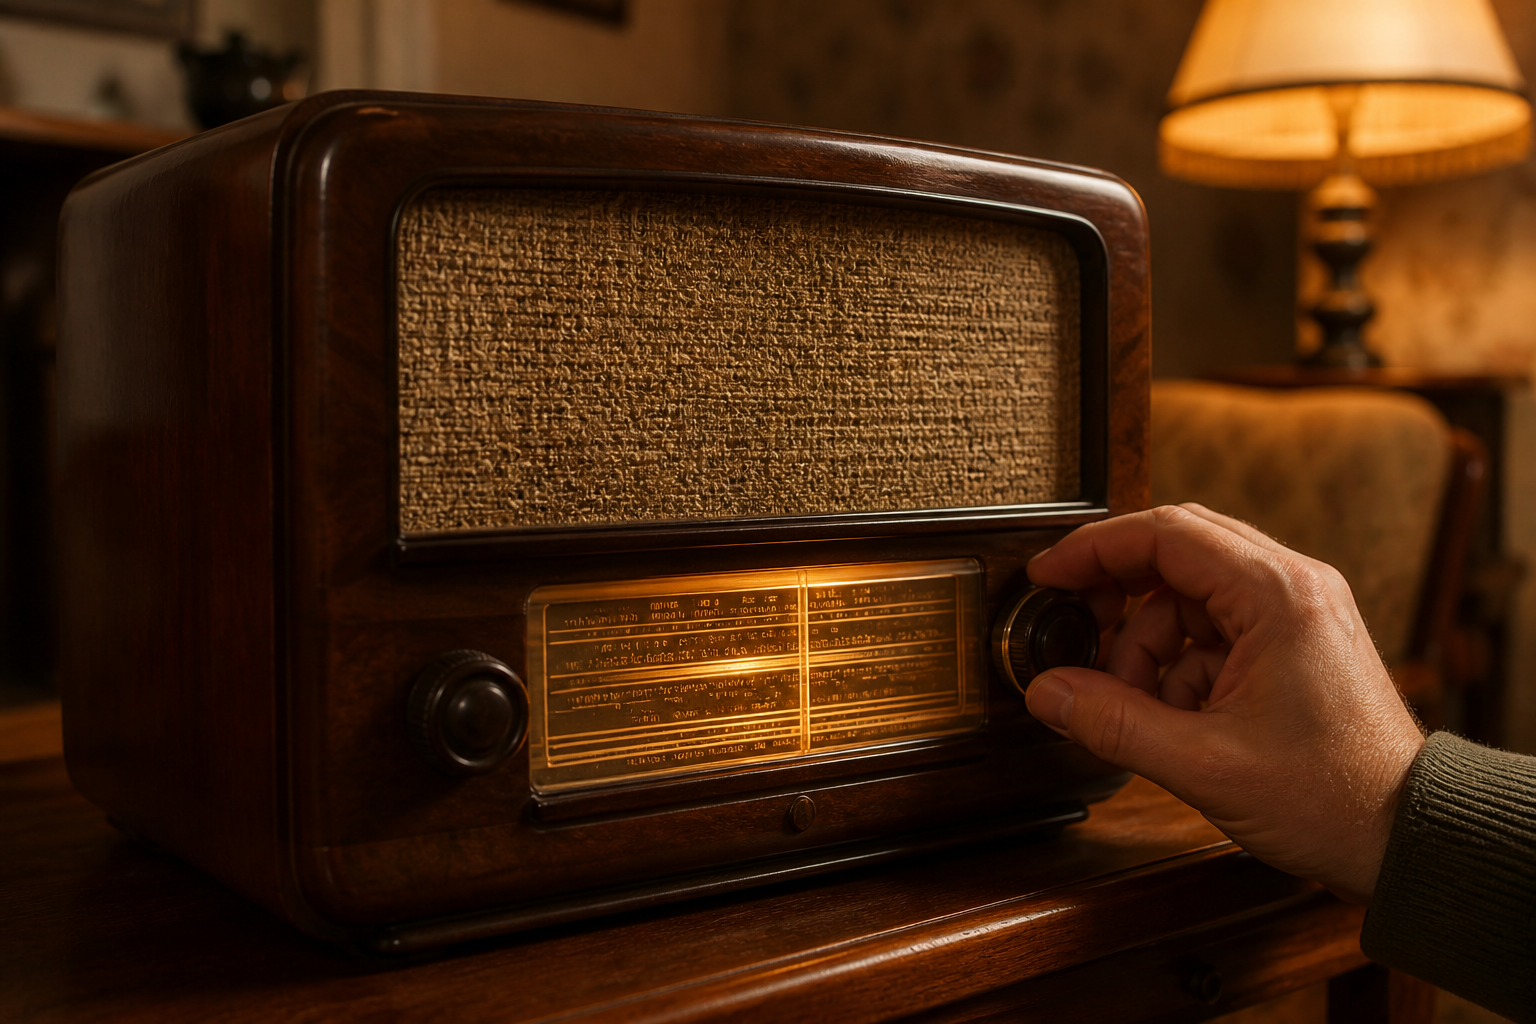
\includegraphics[width=0.55\linewidth]{images/book3/ai/b3-08-vintage-radio-tuning.png}

{\small Tuning a valve radio: turning the knob changes a capacitor, the capacitor sets the resonance frequency of an $LC$ circuit, and the station whose frequency matches is the one heard --- the weekend problem.}
\end{omfigure}

\section{Problem: The resonant radio receiver}

\begin{problem}[{Weekend problem --- a coil, a variable capacitor and
an antenna: how a series resonance picks one station out of a hundred,
multiplies its faint signal by a hundred, and why it cannot be made
arbitrarily selective}]
\label{pb:b1:sinusoidal-impedance:1}
The antenna is modeled by an ideal sinusoidal emf $e(t) = E\cos\omega t$
in series with a coil $L = \qty{200}{\micro H}$, whose wire has
resistance $R = \qty{12.6}{\ohm}$, and a variable capacitor $C$. The
receiver reads the \omterm{def:b1:dc-circuits:voltage}{voltage} across $C$. Later (Part IV) the antenna's
own resistance $R_a = \qty{50}{\ohm}$ is taken into account.

\medskip
\noindent\textbf{Part I --- The resonant current.}
\begin{enumerate}
  \item Write the complex \omterm{def:b1:sinusoidal-impedance:impedance}{impedance} of the series circuit.
  \item Give the \omterm{def:b1:sinusoidal-impedance:complex}{complex amplitude} of the current, then its \omterm{def:b1:wave-propagation:signal}{amplitude}
        $I(\omega)$ and its phase $\varphi_i(\omega)$ relative to $e$.
  \item Show that $I$ is maximal at $\omega_0 = 1/\sqrt{LC}$; give
        $I_{\max}$ and the phase then.
  \item What capacitance tunes $f_0 = \qty{1.000}{MHz}$? Compute
        $L\omega_0$.
  \item Define $Q = L\omega_0/R$ and compute it.
  \item Show that $I/I_{\max} = 1/\sqrt{1 + Q^2(x - 1/x)^2}$ with
        $x = \omega/\omega_0$.
  \item State the sign of $\varphi_i$ below and above resonance and
        interpret (capacitive or inductive behavior).
\end{enumerate}

\medskip
\noindent\textbf{Part II --- Selectivity.}
\begin{enumerate}[resume]
  \item Write the condition defining the two frequencies at which
        $I = I_{\max}/\sqrt2$.
  \item Solve it and show that $\Delta\omega = \omega_2 - \omega_1 =
        \omega_0/Q$.
  \item Compute the bandwidth $\Delta f$ of this receiver.
  \item A second station broadcasts at \qty{1.010}{MHz}, a third at
        \qty{1.020}{MHz}: compute the \omterm{def:b1:wave-propagation:signal}{amplitude} ratio $I/I_{\max}$ for
        each, and the corresponding power ratio in decibels.
  \item AM stations are spaced \qty{9}{} to \qty{10}{kHz} apart. Is the
        receiver selective enough? What would improve it?
  \item The capacitor can be set between \qty{50}{} and \qty{500}{pF}:
        what frequency band does the receiver cover?
\end{enumerate}

\medskip
\noindent\textbf{Part III --- \omterm{def:b1:dc-circuits:voltage}{Voltage} magnification.}
\begin{enumerate}[resume]
  \item Express the \omterm{def:b1:sinusoidal-impedance:complex}{complex amplitude} of the capacitor \omterm{def:b1:dc-circuits:voltage}{voltage} and show
        that at resonance its \omterm{def:b1:wave-propagation:signal}{amplitude} is $QE$.
  \item The antenna emf is $E = \qty{10}{\micro V}$: compute $I_{\max}$
        and the capacitor \omterm{def:b1:dc-circuits:voltage}{voltage} at resonance. Comment.
  \item Show that the coil \omterm{def:b1:dc-circuits:voltage}{voltage} has the same \omterm{def:b1:wave-propagation:signal}{amplitude} and is in
        phase opposition with the capacitor \omterm{def:b1:dc-circuits:voltage}{voltage} at resonance: what
        does the source ``see''?
  \item Compute the energy stored in the circuit at resonance and the
        energy dissipated per period; check that their ratio times
        $2\pi$ is $Q$.
  \item From \cref{ch:b1:transient-regimes}, what is the \omterm{def:b1:transient-regimes:firstorder}{time constant}
        $\tau = 2Q/\omega_0$ of this circuit? Why does a very high $Q$
        eventually distort speech and music (bandwidth of audio:
        about \qty{5}{kHz} for AM)?
  \item If the coil wire resistance doubled (thinner wire), how would
        $Q$, the bandwidth and the capacitor \omterm{def:b1:dc-circuits:voltage}{voltage} change?
\end{enumerate}

\medskip
\noindent\textbf{Part IV --- The antenna's resistance, and power.}
\begin{enumerate}[resume]
  \item With $R_a = \qty{50}{\ohm}$ in series, recompute $Q$, the
        bandwidth and the capacitor \omterm{def:b1:dc-circuits:voltage}{voltage} for $E = \qty{10}{\micro V}$.
        Conclude.
  \item Compute the \omterm{thm:b1:sinusoidal-impedance:power}{average power} delivered by the antenna emf at
        resonance and the fraction dissipated in $R_a$.
  \item The maximum-power theorem would ask for a load resistance equal
        to $R_a$: why is that goal in conflict with selectivity?
  \item Real receivers connect the antenna to a tap on the coil, or
        through a small coupling capacitor. Explain qualitatively what
        this achieves.
  \item Using $P = \tfrac12 UI\cos\varphi$, compute the \omterm{thm:b1:sinusoidal-impedance:power}{power factor} at
        the two half-power frequencies and explain the name
        ``half-power''.
  \item Summarize the design: what $Q$ buys, what it costs, and the
        value chosen for a \qty{1}{MHz} receiver with \qty{10}{kHz}
        channels.
\end{enumerate}
\end{problem}
